\documentclass[journal,12pt,twocolumn]{IEEEtran}


\usepackage{tikz}
\usetikzlibrary{calc,shapes.multipart,chains,arrows}
\usepackage{setspace}
\usepackage{gensymb}
\singlespacing
\usepackage[cmex10]{amsmath}

\usepackage{amsthm}

\usepackage{mathrsfs}
\usepackage{txfonts}
\usepackage{stfloats}
\usepackage{bm}
\usepackage{cite}
\usepackage{cases}
\usepackage{subfig}

\usepackage{longtable}
\usepackage{multirow}

\usepackage{enumitem}
\usepackage{mathtools}
\usepackage{steinmetz}
\usepackage{tikz}
\usepackage{circuitikz}
\usepackage{verbatim}
\usepackage{tfrupee}
\usepackage[breaklinks=true]{hyperref}
\usepackage{graphicx}
\usepackage{tkz-euclide}

\usetikzlibrary{calc,math}
\usepackage{listings}
    \usepackage{color}                                            %%
    \usepackage{array}                                            %%
    \usepackage{longtable}                                        %%
    \usepackage{calc}                                             %%
    \usepackage{multirow}                                         %%
    \usepackage{hhline}                                           %%
    \usepackage{ifthen}                                           %%
    \usepackage{lscape}     
\usepackage{multicol}
\usepackage{chngcntr}

\DeclareMathOperator*{\Res}{Res}

\renewcommand\thesection{\arabic{section}}
\renewcommand\thesubsection{\thesection.\arabic{subsection}}
\renewcommand\thesubsubsection{\thesubsection.\arabic{subsubsection}}

\renewcommand\thesectiondis{\arabic{section}}
\renewcommand\thesubsectiondis{\thesectiondis.\arabic{subsection}}
\renewcommand\thesubsubsectiondis{\thesubsectiondis.\arabic{subsubsection}}


\hyphenation{op-tical net-works semi-conduc-tor}
\def\inputGnumericTable{}                                 %%

\lstset{
%language=C,
frame=single, 
breaklines=true,
columns=fullflexible
}
\begin{document}


\newtheorem{theorem}{Theorem}[section]
\newtheorem{problem}{Problem}
\newtheorem{proposition}{Proposition}[section]
\newtheorem{lemma}{Lemma}[section]
\newtheorem{corollary}[theorem]{Corollary}
\newtheorem{example}{Example}[section]
\newtheorem{definition}[problem]{Definition}

\newcommand{\BEQA}{\begin{eqnarray}}
\newcommand{\EEQA}{\end{eqnarray}}
\newcommand{\define}{\stackrel{\triangle}{=}}
\bibliographystyle{IEEEtran}
\raggedbottom
\setlength{\parindent}{0pt}
\providecommand{\mbf}{\mathbf}
\providecommand{\pr}[1]{\ensuremath{\Pr\left(#1\right)}}
\providecommand{\qfunc}[1]{\ensuremath{Q\left(#1\right)}}
\providecommand{\sbrak}[1]{\ensuremath{{}\left[#1\right]}}
\providecommand{\lsbrak}[1]{\ensuremath{{}\left[#1\right.}}
\providecommand{\rsbrak}[1]{\ensuremath{{}\left.#1\right]}}
\providecommand{\brak}[1]{\ensuremath{\left(#1\right)}}
\providecommand{\lbrak}[1]{\ensuremath{\left(#1\right.}}
\providecommand{\rbrak}[1]{\ensuremath{\left.#1\right)}}
\providecommand{\cbrak}[1]{\ensuremath{\left\{#1\right\}}}
\providecommand{\lcbrak}[1]{\ensuremath{\left\{#1\right.}}
\providecommand{\rcbrak}[1]{\ensuremath{\left.#1\right\}}}
\theoremstyle{remark}
\newtheorem{rem}{Remark}
\newcommand{\sgn}{\mathop{\mathrm{sgn}}}
% \providecommand{\abs}[1]{\left\vert#1\right\vert}
% \providecommand{\res}[1]{\Res\displaylimits_{#1}} 
% \providecommand{\norm}[1]{\left\lVert#1\right\rVert}
% %\providecommand{\norm}[1]{\lVert#1\rVert}
% \providecommand{\mtx}[1]{\mathbf{#1}}
% \providecommand{\mean}[1]{E\left[ #1 \right]}
\providecommand{\fourier}{\overset{\mathcal{F}}{ \rightleftharpoons}}
%\providecommand{\hilbert}{\overset{\mathcal{H}}{ \rightleftharpoons}}
\providecommand{\system}{\overset{\mathcal{H}}{ \longleftrightarrow}}
	%\newcommand{\solution}[2]{\textbf{Solution:}{#1}}
\newcommand{\solution}{\noindent \textbf{Solution: }}
\newcommand{\cosec}{\,\text{cosec}\,}
\providecommand{\dec}[2]{\ensuremath{\overset{#1}{\underset{#2}{\gtrless}}}}
\newcommand{\myvec}[1]{\ensuremath{\begin{pmatrix}#1\end{pmatrix}}}
\newcommand{\mydet}[1]{\ensuremath{\begin{vmatrix}#1\end{vmatrix}}}
\numberwithin{equation}{subsection}
\makeatletter
\@addtoreset{figure}{problem}
\makeatother
\let\StandardTheFigure\thefigure
\let\vec\mathbf
\renewcommand{\thefigure}{\theproblem}
\def\putbox#1#2#3{\makebox[0in][l]{\makebox[#1][l]{}\raisebox{\baselineskip}[0in][0in]{\raisebox{#2}[0in][0in]{#3}}}}
     \def\rightbox#1{\makebox[0in][r]{#1}}
     \def\centbox#1{\makebox[0in]{#1}}
     \def\topbox#1{\raisebox{-\baselineskip}[0in][0in]{#1}}
     \def\midbox#1{\raisebox{-0.5\baselineskip}[0in][0in]{#1}}
\vspace{3cm}
\title{Assignment 1}
\author{Bandi Sai Laxman - EE18BTECH11049}
\maketitle
\newpage
\bigskip
\renewcommand{\thefigure}{\theenumi}
\renewcommand{\thetable}{\theenumi}
Download all files from 
%
\begin{lstlisting}
https://github.com/laxmanbro/gvv_ee4013/tree/main/assign1
\end{lstlisting}
\section{Problem}
Consider the C code fragment given below
\begin{lstlisting}
typedef struct node{
    int data;
    node* next;
} node;

void join(node* m, node* n){
    node* p = n;
    while(p->next != NULL)
        p = p -> next;
    p->next = m ;
}

\end{lstlisting}
Assuming that m and n point to valid NULL-terminated linked lists, invocation of join will ??

\section{Solution}

\subsection{Answer}


As seen from the code above :

The While part in the \textbf{ join function }  take the pointer p to the end of linked list n and then points next to the linked list m. 
\newline

So ,  \textbf{join} will append list m to the end of list n for all inputs .
\newline
\newline
\textbf{ Explanation : }  
\begin{itemize}
    \item Creating two random lists : \textbf{list 1}, \textbf{list 2} .
    
    \begin{figure}[!h]
        \centering
        
        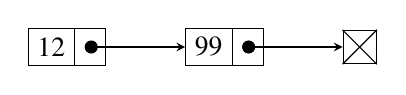
\begin{tikzpicture}[list/.style={rectangle split, rectangle split parts=2,
            draw, rectangle split horizontal}, >=stealth, start chain]
        
          \node[list,on chain] (A) {12};
          \node[list,on chain] (B) {99};
          \node[on chain,draw,inner sep=6pt] (D) {};
          \draw (D.north east) -- (D.south west);
          \draw (D.north west) -- (D.south east);
          \draw[*->] let \p1 = (A.two), \p2 = (A.center) in (\x1,\y2) -- (B);
          \draw[*->] let \p1 = (B.two), \p2 = (B.center) in (\x1,\y2) -- (D);
        \end{tikzpicture}
        
        \caption{List 1} \label{fig:list1}
    \end{figure}
    
    \begin{figure}[!h]
        \centering
        
        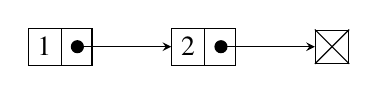
\begin{tikzpicture}[list/.style={rectangle split, rectangle split parts=2,
            draw, rectangle split horizontal}, >=stealth, start chain]
        
          \node[list,on chain] (A) {1};
          \node[list,on chain] (B) {2};
          \node[on chain,draw,inner sep=6pt] (D) {};
          \draw (D.north east) -- (D.south west);
          \draw (D.north west) -- (D.south east);
          \draw[*->] let \p1 = (A.two), \p2 = (A.center) in (\x1,\y2) -- (B);
          \draw[*->] let \p1 = (B.two), \p2 = (B.center) in (\x1,\y2) -- (D);
        \end{tikzpicture}
        
        \caption{List 2} \label{fig:list2}
    \end{figure}
    
    
    \item Calling the \textbf{join(list1, list2)} we get the result as shown in the final Figure
\end{itemize}






\begin{figure}[!h]
\centering

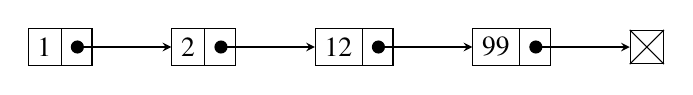
\begin{tikzpicture}[list/.style={rectangle split, rectangle split parts=2,
    draw, rectangle split horizontal}, >=stealth, start chain]

  \node[list,on chain] (A) {1};
  \node[list,on chain] (B) {2};
  \node[list,on chain] (E) {12};
  \node[list,on chain] (F) {99};
  \node[on chain,draw,inner sep=6pt] (D) {};
  \draw (D.north east) -- (D.south west);
  \draw (D.north west) -- (D.south east);
  \draw[*->] let \p1 = (A.two), \p2 = (A.center) in (\x1,\y2) -- (B);
  \draw[*->] let \p1 = (B.two), \p2 = (B.center) in (\x1,\y2) -- (E);
  \draw[*->] let \p1 = (E.two), \p2 = (E.center) in (\x1,\y2) -- (F);
  \draw[*->] let \p1 = (F.two), \p2 = (F.center) in (\x1,\y2) -- (D);
\end{tikzpicture}

\caption{Final Result } \label{fig:tree1}
\end{figure}

 So the list1 will get appended to list2 . 
 
 \subsection{Time Complexity Analysis}
 
 Considering the part of code below . 
 
 \begin{lstlisting}
while(p->next != NULL)
        p = p -> next;
    p->next = m ;

\end{lstlisting}

The while loop terminates after pointer p reaches NULL , which happens at the end of linked list 2.
Assuming Length of list2 is n . 
\newline
The worst Case Time Complexity of above code is  $\mathcal{O}(n)$.
 
 
 

 


\end{document}
